% Options for packages loaded elsewhere
\PassOptionsToPackage{unicode}{hyperref}
\PassOptionsToPackage{hyphens}{url}
%
\documentclass[
  ignorenonframetext,
]{beamer}
\usepackage{pgfpages}
\setbeamertemplate{caption}[numbered]
\setbeamertemplate{caption label separator}{: }
\setbeamercolor{caption name}{fg=normal text.fg}
\beamertemplatenavigationsymbolsempty
% Prevent slide breaks in the middle of a paragraph
\widowpenalties 1 10000
\raggedbottom
\setbeamertemplate{part page}{
  \centering
  \begin{beamercolorbox}[sep=16pt,center]{part title}
    \usebeamerfont{part title}\insertpart\par
  \end{beamercolorbox}
}
\setbeamertemplate{section page}{
  \centering
  \begin{beamercolorbox}[sep=12pt,center]{part title}
    \usebeamerfont{section title}\insertsection\par
  \end{beamercolorbox}
}
\setbeamertemplate{subsection page}{
  \centering
  \begin{beamercolorbox}[sep=8pt,center]{part title}
    \usebeamerfont{subsection title}\insertsubsection\par
  \end{beamercolorbox}
}
\AtBeginPart{
  \frame{\partpage}
}
\AtBeginSection{
  \ifbibliography
  \else
    \frame{\sectionpage}
  \fi
}
\AtBeginSubsection{
  \frame{\subsectionpage}
}
\usepackage{amsmath,amssymb}
\usepackage{lmodern}
\usepackage{iftex}
\ifPDFTeX
  \usepackage[T1]{fontenc}
  \usepackage[utf8]{inputenc}
  \usepackage{textcomp} % provide euro and other symbols
\else % if luatex or xetex
  \usepackage{unicode-math}
  \defaultfontfeatures{Scale=MatchLowercase}
  \defaultfontfeatures[\rmfamily]{Ligatures=TeX,Scale=1}
\fi
% Use upquote if available, for straight quotes in verbatim environments
\IfFileExists{upquote.sty}{\usepackage{upquote}}{}
\IfFileExists{microtype.sty}{% use microtype if available
  \usepackage[]{microtype}
  \UseMicrotypeSet[protrusion]{basicmath} % disable protrusion for tt fonts
}{}
\makeatletter
\@ifundefined{KOMAClassName}{% if non-KOMA class
  \IfFileExists{parskip.sty}{%
    \usepackage{parskip}
  }{% else
    \setlength{\parindent}{0pt}
    \setlength{\parskip}{6pt plus 2pt minus 1pt}}
}{% if KOMA class
  \KOMAoptions{parskip=half}}
\makeatother
\usepackage{xcolor}
\IfFileExists{xurl.sty}{\usepackage{xurl}}{} % add URL line breaks if available
\IfFileExists{bookmark.sty}{\usepackage{bookmark}}{\usepackage{hyperref}}
\hypersetup{
  pdftitle={Introduction to Statistics},
  pdfauthor={Adejumo Ridwan Suleiman},
  hidelinks,
  pdfcreator={LaTeX via pandoc}}
\urlstyle{same} % disable monospaced font for URLs
\newif\ifbibliography
\usepackage{graphicx}
\makeatletter
\def\maxwidth{\ifdim\Gin@nat@width>\linewidth\linewidth\else\Gin@nat@width\fi}
\def\maxheight{\ifdim\Gin@nat@height>\textheight\textheight\else\Gin@nat@height\fi}
\makeatother
% Scale images if necessary, so that they will not overflow the page
% margins by default, and it is still possible to overwrite the defaults
% using explicit options in \includegraphics[width, height, ...]{}
\setkeys{Gin}{width=\maxwidth,height=\maxheight,keepaspectratio}
% Set default figure placement to htbp
\makeatletter
\def\fps@figure{htbp}
\makeatother
\setlength{\emergencystretch}{3em} % prevent overfull lines
\providecommand{\tightlist}{%
  \setlength{\itemsep}{0pt}\setlength{\parskip}{0pt}}
\setcounter{secnumdepth}{-\maxdimen} % remove section numbering
\ifLuaTeX
  \usepackage{selnolig}  % disable illegal ligatures
\fi

\title{Introduction to Statistics}
\author{Adejumo Ridwan Suleiman}
\date{March 22, 2005}

\begin{document}
\frame{\titlepage}

\hypertarget{introduction-to-statistics}{%
\section{Introduction to Statistics}\label{introduction-to-statistics}}

\begin{frame}{What is Statistics?}
\protect\hypertarget{what-is-statistics}{}
\begin{itemize}
\tightlist
\item
  Statistics is the collection, organizing and analysing of data.
\end{itemize}
\end{frame}

\begin{frame}{Is Data Science Statistics in Disguise?}
\protect\hypertarget{is-data-science-statistics-in-disguise}{}
\begin{itemize}
\tightlist
\item
  Unlike Statistics, Data Science is an interdisciplinary field
  consisting of Mathematics, Statistics, Computer Science and Domain
  Knowledge.
\end{itemize}
\end{frame}

\begin{frame}{Types of Data}
\protect\hypertarget{types-of-data}{}
\begin{itemize}
\tightlist
\item
  Data can be classified into two types

  \begin{itemize}
  \tightlist
  \item
    Based on Measurement scale\\
  \item
    Based on Time Period
  \end{itemize}
\end{itemize}
\end{frame}

\begin{frame}{Based on Measurement Scale}
\protect\hypertarget{based-on-measurement-scale}{}
\begin{itemize}
\tightlist
\item
  Qualitative Data

  \begin{itemize}
  \tightlist
  \item
    Nominal Data e.g sex
  \item
    Ordinal Data e.g temperature level; High, Medium and Low
  \end{itemize}
\item
  Quantitative Data

  \begin{itemize}
  \tightlist
  \item
    Ratio e.g weight
  \item
    Interval e.g temperature in degreee celsius
  \end{itemize}
\end{itemize}
\end{frame}

\begin{frame}{Based on Time Period}
\protect\hypertarget{based-on-time-period}{}
\begin{itemize}
\tightlist
\item
  Cross-Sectional Data e.g number of viewers for different youtube
  genres in the year 2021
\item
  Time Series Data e.g number of viewers for Sport channels on youtube
  from the year 2014-Date.
\end{itemize}
\end{frame}

\begin{frame}{}
\protect\hypertarget{section}{}
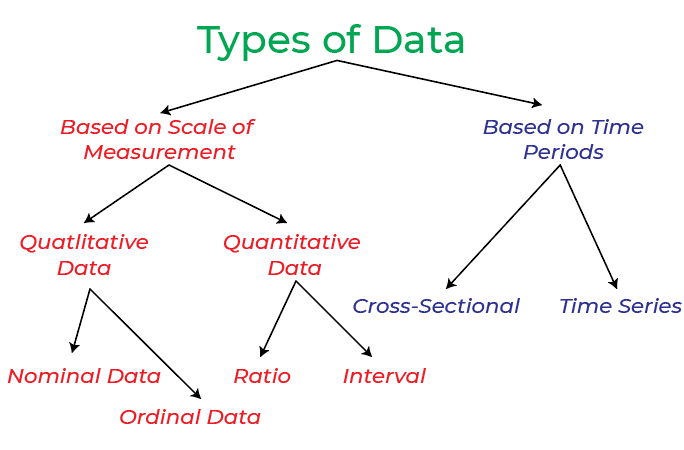
\includegraphics{"/types_of_data.png"}
\end{frame}

\end{document}
